\documentclass[12pt]{article}
\usepackage{graphicx}
\usepackage{amsmath}
\usepackage{geometry}
\usepackage{listings}
\usepackage{color}
\usepackage{array}
\usepackage{hyperref}
\usepackage{url}

\geometry{a4paper, margin=1in}

\definecolor{mygreen}{rgb}{0,0.6,0}
\definecolor{mygray}{rgb}{0.5,0.5,0.5}
\definecolor{mymauve}{rgb}{0.58,0,0.82}

\lstset{
	language=C++,
	basicstyle=\ttfamily\small,
	numbers=left,
	numberstyle=\tiny,
	stepnumber=1,
	numbersep=10pt,
	tabsize=4,
	breaklines=true,
	captionpos=b,
	keywordstyle=\color{blue}\bfseries,
	commentstyle=\color{mygray},
	stringstyle=\color{red}
}

\begin{document}
			\begin{titlepage}
				\centering
				
				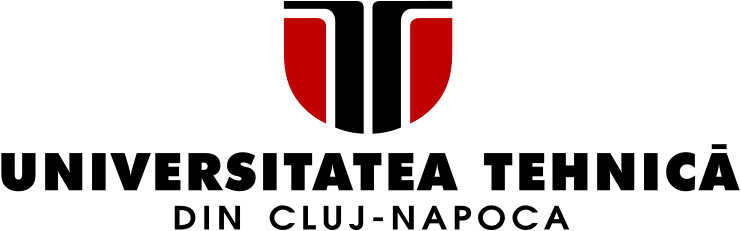
\includegraphics[width=0.4\textwidth]{logo.png}\\
				\vspace*{6cm}
				
				\Huge
				\textbf{Project Title}
				
				\vspace{0.5cm}
				\Large
				Project Documentation
				
				\vspace{1.5cm}
				
				\textbf{Grad Laurentiu-Calin}\\
				\text{Group 30435}
				
				\vfill
				
				\Large
				Computer Science\\
				December, 2024\\
				
			\end{titlepage}
			
	\newpage
	\tableofcontents
	\newpage
	
	\section{Introduction: Purpose and Motivation}
	\begin{itemize}
		\item Why did you choose this project?
		\item What scope do you want to fulfill?
		\item Is it a well-known idea that you wanted to implement for yourself? Or did you want to try something new because no existing solution satisfied you?
	\end{itemize}
	
	
	
	\section{Bibliographic Research}
	\begin{itemize}
		\item Find some existing solutions for your idea (or close to your idea) and compare them.
		\item Resume to a very short description of the solutions and compare them from different perspectives: power consumption, difficulty to implement, cost of resources and implementation, adaptation to user's needs, etc.
	\end{itemize}
	
	There are multiple implementation and design project ideas related to greenhouses, temperature or humidity monitoring in different media that are available on-line, some interesting ones that I have encountered are: \cite{aleixj}, \cite{ejsh}, \cite{sgarro}. However, I chose to implement this in my own way, without taking inspiration from any of these. Consequently, my research focused on searching, finding, purchasing and working with sensors, development boards, electrical circuits and diagrams. 
	
	A wide variety of temperature or temperature \& humidity sensors is available on the market. I set on three of them:
	
	\begin{itemize}
		\item HR202 $\rightarrow$ humidity sensor.
		\item DHT11 $\rightarrow$ temperature sensor.
		\item DHT22 $\rightarrow$ temperature \& humidity sensor.
	\end{itemize}
	
	The core differences between the above mentioned sensors are summarized in the table below:
	
	\begin{table}[h]
		\centering
		\begin{tabular}{|m{3cm}|>{\centering\arraybackslash}m{3cm}|>{\centering\arraybackslash}m{3cm}|>{\centering\arraybackslash}m{3cm}|}
			\hline 
			\textbf{Feature} & \textbf{HR202} & \textbf{DHT22} & \textbf{DHT11} \\
			\hline
			\textbf{Type} & Resistive Humidity Sensor & DIgital Humidity and Temperature Sensor & Digital Humidity and Temperature Sensor \\
			\hline
			\textbf{Humidity Range} & 20\% to 95\% RH & 0\% to 100\% RH & 5\% to 95\% RH \\
			\hline
			\textbf{Temperature Range} & 0°C to 60°C & -40°C to 80°C & -20°C to 60°C \\
			\hline
			\textbf{Humidity Accuracy} & ±15\% RH & ±2\% to ±5\% RH & ±5\% RH \\
			\hline
			\textbf{Temperature Accuracy} & \textit{Undefined} & ±0.5°C & ±2°C \\
			\hline
			\textbf{Output} & Digital & Digital & Digital \\
			\hline
			\textbf{Power Supply} & 3.3V - 5V DC & 3V - 6V DC & 3V - 5.5V DC \\
			\hline
			\textbf{Communication} & Analog & One-wire & One-wire \\
			\hline
			\textbf{Response time} & Not Specified & ~2 seconds & ~2 seconds \\
			\hline
			\textbf{Common applications} & Weather monitoring, Dew detection & Weather stations, Greenhouse monitoring & Home weather stations, Environmental monitoring \\
			\hline
		\end{tabular}
		\caption{Comparison of \textbf{HR202}, \textbf{DHT22}, and \textbf{DHT11} sensors}
		\label{tab::sensor_comparison}
	\end{table}
	
	\clearpage
	
	\section{Proposed Solution and Implementation}
	\begin{itemize}
		\item Overall description of the solution chosen.
		\item Theoretical description of your algorithm(s).
		\item Implementation:
		\begin{itemize}
			\item Hardware: draw a circuit of your hardware parts and their connections.
			\item Software: describe the relevant functions and how they work together. 
		\end{itemize}
	\end{itemize}
	
	I have chosen to implement my project in a bottom-up manner, meaning that I started with small parts that had nothing to do with each other at first glance. Once all these modules had been designed, implemented and tested, I moved to creating the inter-component logic. The main advantage my approach offered was to let me think in object-oriented style. Thus, each component (printed circuit boards, simple LED-s, temperature or humidity sensors) was wrapped inside an abstract object (class). Being a relatively complex project thanks to the amount of components that have different behaviors, the development process was accelerated because I had access to the high-level abstraction mechanisms provided by C++. By following the \textit{SOLID} principles and some \textit{good practice} industry rules, the final form of the source code appears to me as maintainable, clear to use and improve, and most importantly free of bugs, useless code and verbosity.
	
	\subsection{The DHT22 Sensor}
	
	\textit{DHT22} is a temperature and humidity sensor. It is a really popular measuring device because it has a low production cost and is easy to use. Thanks to this popularity a lot of open-source libraries that implement high-level operations already exist: \textit{SimpleDHT, Adafruit Unified Library, etc}.
	
	\begin{figure}[ht]
		\centering
		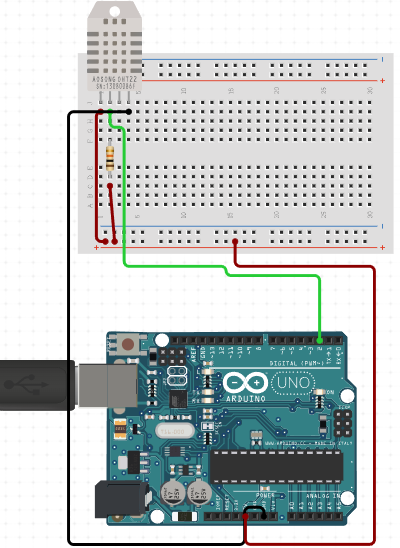
\includegraphics[width=0.4\textwidth]{diag_dht22.png}
		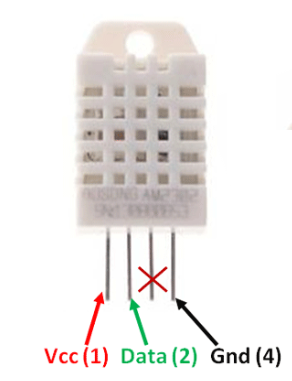
\includegraphics[width=0.4\textwidth]{dht.png}
		\caption{The DHT22 sensor Arduino diagram and a close-up of the component}
		\label{fig:DHT22}
	\end{figure}
	
	\begin{lstlisting} [caption = C++ class definition of the DHT22 sensor]
#include <stdint.h>
#include <Adafruit_Sensor.h>
#include <DHT.h>
#include <DHT_U.h>

class DHT22Sensor {
	public:
		DHT22Sensor() : dht(12, DHT22) {};
		void setupSensor();
		void sensorLoop();
	private:
		// the pin on the Arduino board that is 
		// connected to the data pin of the DHT22
		const int dataPin = 12;
		// sensor wrapper provided by 
		// Adafruit_sensor.h
		DHT_Unified dht;
		// how many miliseconds we have to wait 
		//to read data from the sensor again
		uint32_t delayMS;
};
	\end{lstlisting}
	
	\clearpage
	
	\subsection{RGB led}
	
	A simple common cathode RGB led.
	
	\begin{figure}[ht]
		\centering
		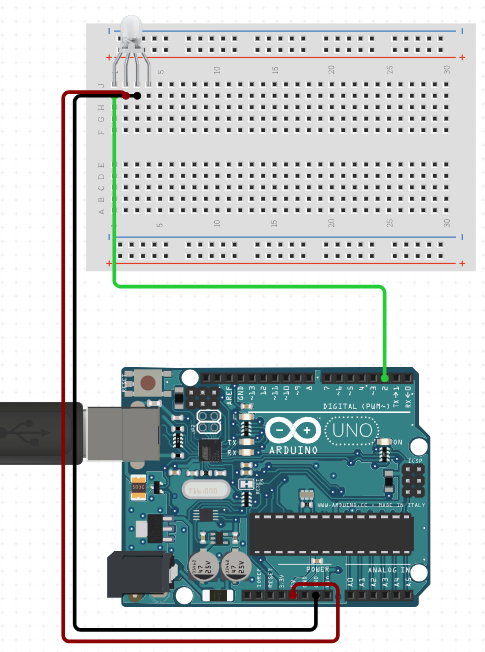
\includegraphics[width=0.4\textwidth]{diag_led.png}
		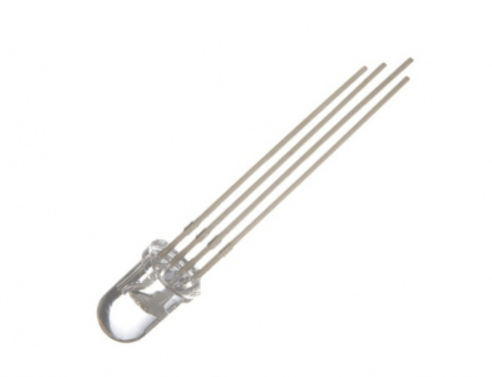
\includegraphics[width=0.4\textwidth]{led.png}
		\caption{The RGB led Arduino diagram and a close-up of the component}
		\label{fig:rgb_led}
	\end{figure}
	
	\begin{lstlisting}[caption = C++ class definition of the RGB LED module]
#include "Types.hpp"
#include "Arduino.h"

class LED
{
	public:
		explicit LED(Color newColor) : color(newColor) {};
		void setupLed() const;
		int getRedPin() const { return redPin; };
		int getGreenPin() const { return greenPin; };
		int getBluePin() const { return bluePin; };
		Color getColor() const { return color; };
		void setColor(Color newColor) { color = newColor; };
		void displayColor() const;
	private:
		const int redPin{11};   // PWM pin
		const int greenPin{10}; // PWM pin
		const int bluePin{9};   // PWM pin
		Color color;
};
	\end{lstlisting}
	
	\clearpage
	
	\subsection{8-LED module}
	
	This is a fairly basic printed circuit board that houses 8 LED-s in common anode configuration.

	\begin{figure}[ht]
		\centering
		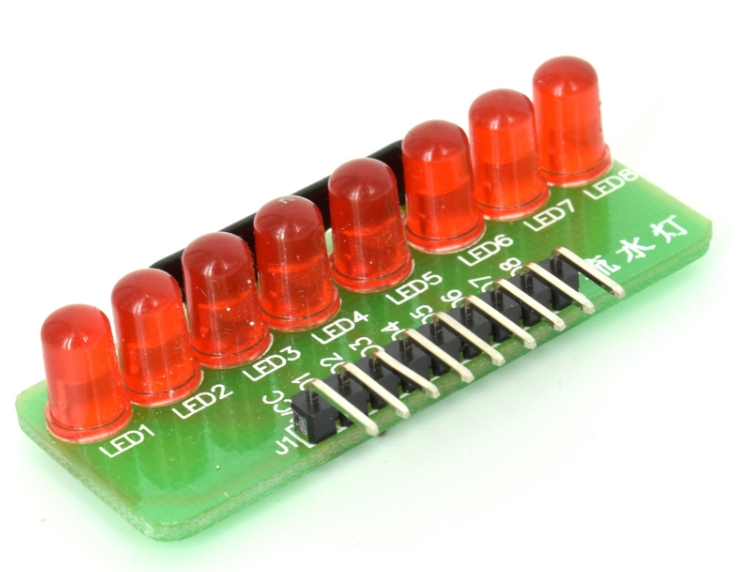
\includegraphics[width=0.4\textwidth]{leds.png}
		\caption{The led module printed circuit board}
		\label{fig:led_module}
	\end{figure}

	\begin{lstlisting}[caption = C++ class definition of the LED module]
#include "Arduino.h"

class LedModule
{
	public:
		LedModule() {};
		void setupLedModule() const;
		int getLedPin(int index) const;
		void turnOnLed(int index) const;
		void turnOffLed(int index) const;
	private:
		// the 8 pins of the Arduino board that are connected
		// to the 8 individual cathodes of the led module
		const int leds[8]{1, 2, 3, 4, 5, 6, 7, 8};
		const int numberOfLeds{8};
};
	\end{lstlisting}
	
	\clearpage
	
	\subsection{Buzzer}
	Another basic component that emits sounds with respect to a channel that supports PWM. 
	
	\footnotetext[1]{\label{fn:buzzer} The PCB I use has an integrated transistor and resistance meaning that interfacing with the board is much simpler: 2 power connections (GND and VCC) and a data wire.}
	
	\begin{figure}[ht]
		\centering
		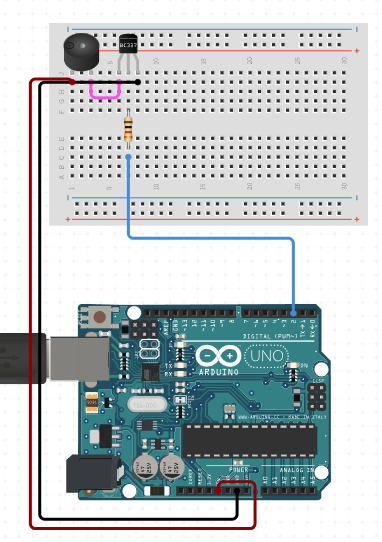
\includegraphics[width=0.4\textwidth]{diag_buzzer.png}
		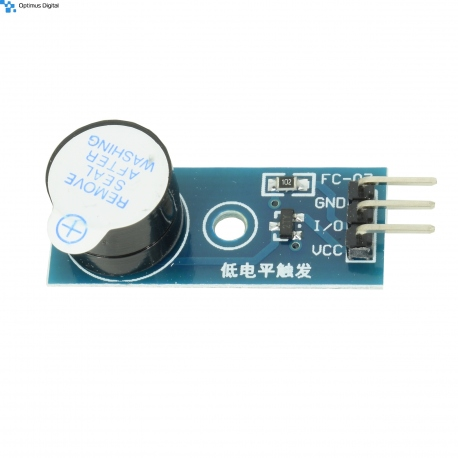
\includegraphics[width=0.4\textwidth]{buzzer.jpg}
		\caption{The diagram connection of a simple buzzer and a close-up of the component\textsuperscript{\ref{fn:buzzer}}}
		\label{fig:buzzer}
	\end{figure}
	
	\begin{lstlisting}
#include "Arduino.h"
#include "Pitches.hpp"
#include "Types.hpp"

class Buzzer
{
	public:
		Buzzer() {};
		void setupBuzzer() const;
		void turnOn(int noteFrequency, Notes duration);
		void turnOff();
		void buzzerLoop();
	private:
		// PWM Arduino Pin that is connected to the data pin
		// of the buzzer
		const int dataPin{3};
		const float pauseStretch{1.3f};
};
	\end{lstlisting}
	
	\begin{figure}[ht]
		\centering
		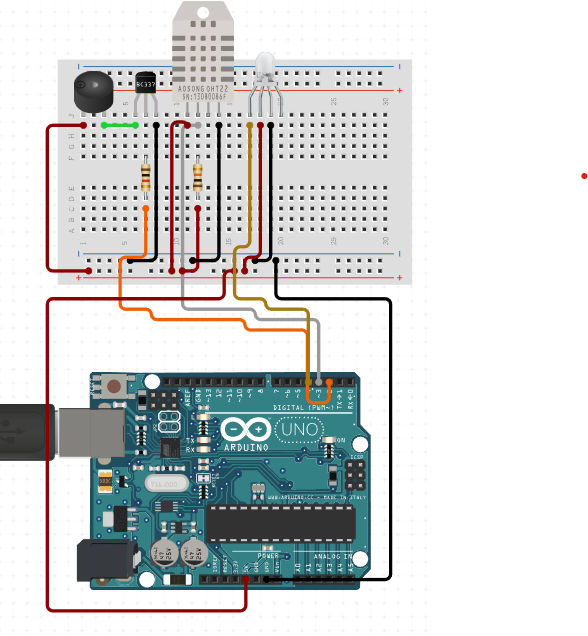
\includegraphics[width=0.4\textwidth]{diag_full1.png}
		\caption{Arduino diagram for different phases of the project}
		\label{fig:sys_diag}
	\end{figure}
	
	\clearpage
	
	\section{Testing and Validation}
	\begin{itemize}
		\item What problems did you encounter while implementing your solution?
		\item Make tables to compare your project's behavior when you changed some aspects in the environment.
		\item Describe the phases your project went through.
	\end{itemize}
	
	\section{Conclusion}
	\begin{itemize}
		\item Was your purpose fulfilled? 
		\item How can your solution help others? 
		\item How can it practically be improved?
	\end{itemize}
	
	\bibliographystyle{plain} 
	\bibliography{references}
	
\end{document}
